%Introduce and discuss the design decisions that you made during this project.
%Highlight why individual choices are important and/or necessary. Discuss
%how the design fits together.

%This section is usually 5-10 pages.

%%%%%%%%%%%%%%%%%%%%%%%%%%%%%%%%%%%%%%%%%%%%%%%%%%%%%%%%%%%%

%Multiple individual contributions:
%* Ensemble aggregation methods to evaluate model uncertainty.
%* Experiments on the effect of class imbalance on UQ performance.
%* OOD evaluation of models using adversarial perturbations

%2nd part:
%  - Focus on NLP and hallucinations of LM.=

This chapter first covers the models implemented in the standardised UQ package to estimate data and model uncertainty. Then, models specific to NLP, sequence-to-sequence and graph-to-text models are described.  


\section{General uncertainty quantification models} \label{design:uq-models}

Due to the \textit{scikit-learn} constraints of the package to be developed, the following base models are considered: Logistic Regression, Linear Regression, Gaussian Processes, Gradient-Boosted Trees, Random Forest and  Gaussian Mixture Models. In this work, a base model corresponds to a model for which uncertainty quantification shall be performed. 

%\subsection{Data UQ}

For classification, data uncertainty is measured by the entropy of the prediction distribution $\Entropy_i = - \sum_k \log p_{i,k}$ for data point $x_i$. For regression, one of probabilistic regression (cf. \ref{model:probabilistic-learning}), ensemble-based models (cf. \ref{model:ensembles}) or quantile regression (cf. \ref{model:quantile-regression}) is considered depending on the base model used. 

To estimate model uncertainty, more than one standalone model is required. To solve this issue, ensembles are used in this work, as shown in section \ref{section:background:ensembles}. Different types of ensembles are considered: seed ensemble, hyper-parameter ensemble, bagging ensemble and adversarial ensemble. The latter is the only model not introduced in section \ref{model:ensembles}.

\section{Adversarial ensembles} \label{section:design:adversarial}
Consider a set of adversarial attacks $\mathcal{A} = \{A_1, \ldots, A_L\}$ and the adversarial training procedure in algorithm \ref{alg:adversarial-training}. Ensemble adversarial training trains $M$ of these models independently and aggregates their predictions. Attacks are defined as functions that produce perturbations $\delta = A(D)$ when given as input a dataset $D = (X,Y) = \{(x_i, y_i)\}_i$. Some attacks do not require the $\{y_i\}_i$ labels.

\begin{algorithm}
\caption{Adversarial training.}\label{alg:adversarial-training}
\begin{algorithmic}

\Require $f_{\theta}$ and $D_{train} = (X,Y)$ \Comment{model function and training data set}
\Require $\mathcal{A}$ \Comment{set of adversarial attacks}
\Require $\eta$ \Comment{number of adversarial training epochs}
%\State $y \gets []$
\For{$i \gets 1$, $\eta$}
    \State $A = Sample(\mathcal{A})$
    \State $\delta = A(D_{train})$
    \State $\Tilde{X} = X + \delta$  
    \State $train(f_{\theta}, \Tilde{X})$ \Comment{train the model for a few epochs}
\EndFor
\end{algorithmic}
\end{algorithm}

However, an attack on such ensembles can not be carried out using gradient methods on the ensemble as a whole. Instead, attacks have to be placed on individual members of the ensemble. Let $\mathcal{A} = \{A_1, \ldots, A_M\}$ be a set of $M$ attacks, each placed on a single model, i.e. $A_m$ generates perturbations fooling model $f_m$. An ensemble attack can be defined as:
$$
\delta_{ensemble} = A_{ensemble}(D) = g(A_1(D), \ldots A_M(D)) = g(\delta_1, \ldots, \delta_M)
$$

$g$ is an aggregation function which can either be the mean, the median, the maximum, or a uniform random sample, etc. For instance:
$
g_{mean}(\delta_1, \ldots, \delta_M)_d = \frac{1}{M} \sum_i \delta_{i,d}
$
or
$
g_{random}(\delta_1, \ldots, \delta_M) = \delta_{W}\; \text{such that} \;  W \sim Uniform(1,M)
$.


\section{UQ models for graph-to-text} \label{design:UQ-models-G2T}

Sequence-to-sequence transformers such as T5 are composed of an encoder and a decoder part. For our use case, the quantity of interest is the uncertainty of the natural language generation task. Assuming that the encoder builds an accurate embedding for the input graph, the focus can be placed on the decoding phase with respect to UQ. As declared in section \ref{intro:problem-section}, the aim of UQ models is to produce uncertainty scores at token-level for the prediction texts. Of course, these sources can easily be aggregated at higher granularity, e.g. words or sentences. 

\subsection{Prediction entropy sequence} \label{models:entropy-sequence}

In UQ for classification, the primary quantity of interest is the entropy of the prediction distribution, i.e. SoftMax outputs for the target variable. In text generation, prediction is not about a single variable but rather a causal sequence of tokens $\{t_j\}_{j=1}^L$ defined in the simple case of greedy decoding, by 
$
    t_j = \argmax_k \; p_{j,k} = \argmax_k \; P[t_k \mid t_{j-1}, t_{j-2}, \ldots, t_{0}]
$.

The equivalent notion of predicted entropy for text generation is the predicted entropy sequence $\{\Entropy_j\}_{j=1}^L$, defined as $\Entropy_j = \Entropy(p_j) = - \sum_k p_{j,k} \log p_{j,k} $.

\subsection{Ensembles}

As earlier sections demonstrate, ensembles are essential to improve uncertainty quantification models. The following types are considered:

\begin{enumerate}
    \item Deep ensemble: multiple independent copies of a base model are trained on the same dataset, using different seeds. In previous sections, this model was also called seed ensemble. 
    \item Dropout ensemble: T5 was pre-trained using dropout. If fine-tuning is performed using the same dropout strategy, dropout can be used at test time to generate multiple predictions and approximate model uncertainty (cf. section \ref{model:scalable-DL}).
    \item \label{model:graph-encoding-ensemble} Graph encoding ensemble: the first step of the current graph-to-text pipeline is to linearise the graph into an ordered sequence of edges. This sequence is then passed to the T5 sequence-to-sequence model to generate the final textual representation of the graph. However, there are $|E|!$ possible orderings, which all represent the same graph. Therefore, ensembling a few predictions based on different linearisation can provide a further method to quantify the uncertainty related to the input graph.
\end{enumerate}

However, it remains to discuss how these different predictions should be aggregated to produce an uncertainty score. The aggregation can be performed at two different levels. First, consider the aggregation at text-level. Each model $m$ predicts a natural textual output $T^m$, and each of them is composed of an independent sequence of tokens $\{t_j^m\}_{j=1}^{n_m}$. One possible output aggregation strategy is explained below:
    \begin{enumerate}
        \item Choose a reference output $T^*$ among $\{T^m\}_{m=1}^M$. For instance, it could be the text with the highest probability (or lowest perplexity).
        \item For each output $T^m$ where $m \not= *$, use a string sub-sequence matching algorithm between $T^*$ and $T^m$ to highlight which characters/tokens of $T^m$ are in agreement with $T^*$. Let $a_j^m = 1$ if that is the case and $a_i^m = 0$ otherwise.
        \item For each character/token $t_j^m$, the uncertainty score is defined as $\frac{1}{M} \sum a_i^m$.
    \end{enumerate}
This approach is only valid under the assumption that the outputs $\{T^m\}_{m=1}^M$ are very similar, which is the case for some of the datasets considered in this work. Several tests were conducted on this aggregation type, and we realised that many errors were introduced during the matching phase. In the end, the alternative token-level aggregation was selected as the method of choice. In this approach, consider the prediction token distributions produced by each ensemble member.

$$
p_{j,k}^m = P[t_k^m \mid t_{j-1}, t_{j-2}, \ldots, t_{0}] \;\;\; \forall k=0,1,\ldots, |V|
$$

They can be averaged to create the average ensemble distribution $\bar{p}_{j,k} = \frac{1}{M} \sum_m p_{j,k}^m$
and the associated entropy sequence $\{H(\bar{p}_{j}) \}_{j=1}^L$. To construct the individual member distributions $p_{j,k}^m$, a reference model, e.g. $m=1$ is first selected to generate a reference predicted token sequence $T^1 = \{t_{j}^1\}_{j=1}^L$ with associated token distribution $\{p_{j,k}^1\}_{j,k}$. The other members $m=2, \ldots, M$ are then forced to regenerate $T^1$ using the modified decoding procedure available in algorithm \ref{alg:targeted-decoding}, named targeted decoding. To implement this method, it is required to modify the transformers library's decoding algorithms (greedy search, beam search, etc.). More generally, targeted decoding can be valuable in studying the predicted probability distribution of user-defined token sequences instead of relying on the model to generate them. 

\begin{algorithm}
\caption{Targeted decoding.}\label{alg:targeted-decoding}
\begin{algorithmic}

\Require $f$, $X$,  $t_j \;\forall \; j=1, \ldots, j=L$   \Comment{model function, input sequence and target tokens.}
\State $y$, $p$, $h \gets EmptyList$
\State $y.append(StartSequenceToken)$
\State $j \gets 1$
\While{$j \leq L$}
    \State $y.append(t_j)$  \Comment{Generate the same token as the target tokens}
    \State $s \gets f_j(X, y)$  \Comment{Causal token prediction using input and partial output}
    \State $p_j \gets Softmax(s)$
    \State $p.append(p_j)$
    \State $h.append(Entropy(p_j))$ \Comment{Compute entropy}
    \State $j \gets j + 1$
\EndWhile
\State \Return $y$, $p$, $h$
\end{algorithmic}
\end{algorithm}


\subsection{Synthetic data creation for token-level hallucination detection} \label{design:synthetic-hallucination-data}


\begin{figure}[t]
    \centering
    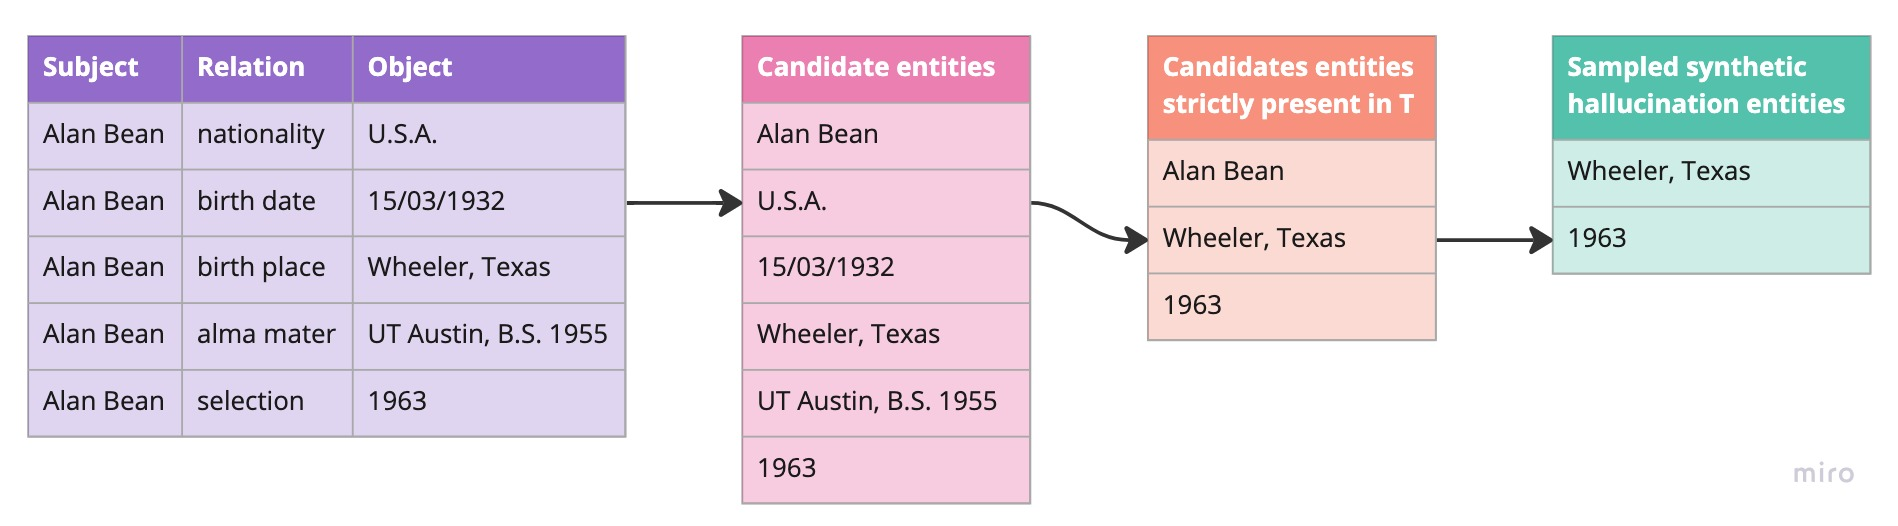
\includegraphics[scale=0.23]{figures/design/synthetic/hallu_ents_selection.jpg}
    \caption{Phase (a). Synthetic hallucination entities generation, i.e. $\tilde{C}_G$.}
    \label{fig:synthetic-ents-selection}
\end{figure}

In this section, the focus is placed on graph-to-text datasets. Modified versions of the datasets introduced in section \ref{section:datasets} are built to study hallucinations due to missing edge information. Unlike other NLP tasks, hallucinations in data-to-text models can often be checked using the input data, which acts as an internal knowledge base. Hallucinations are defined at token-level: for each token $t_j$ in the prediction text $T$, a binary label $a_j$ is assigned. It indicates whether it corresponds or not to a hallucination. 

Zhou et al.\cite{HallucationDetectionUsingSyntheticData} proposed a method to generate a similar synthetic labelled dataset for token-level hallucination in a machine translation context. However, they introduced hallucinations by updating some tokens in the prediction texts. A different approach is undertaken in this work that does not require any modification to the reference or prediction texts. The hallucinations are introduced by dropping meaningful pieces of information from the input sequence so that factual errors naturally occur in the output sequence. 

% The intuition is that some information necessary to generate a piece of text has been removed from the input data. Therefore, concerning the new dataset, this information corresponds to a hallucination. 

%The synthetic data creation is defined as follows
Consider a graph and text pair $(G, T)$. The first phase of the synthetic data generation process is to create $C_G$, a set of candidate hallucination entities from $G$. It consists of all subjects and objects contained in the edges of $G$, i.e. $C_{G} = \bigcup_{e \in G} \{subject(e), object(e)\}$. Then entities that are not strictly present in $T$ are filtered out. For example, if a date $15/03/1932$ is a candidate entity but is only present in $T$ in a written format such as March 15, 1932, it will not be considered anymore. This ensures a low matching error between the entities in $C_G$ and the entities in $T$. From $C_G$,  $K < |C_G|$ entities are sampled and stored in $\Tilde{C}_G$. The latter is the final hallucination entity set. Sub-sampling avoids creating an overly large number of hallucinations which would lead to inconsistencies in the dataset. Figure \ref{fig:synthetic-ents-selection} illustrates this process via the graph-to-text example of section \ref{background:G2T}.

\begin{figure}
    \centering
    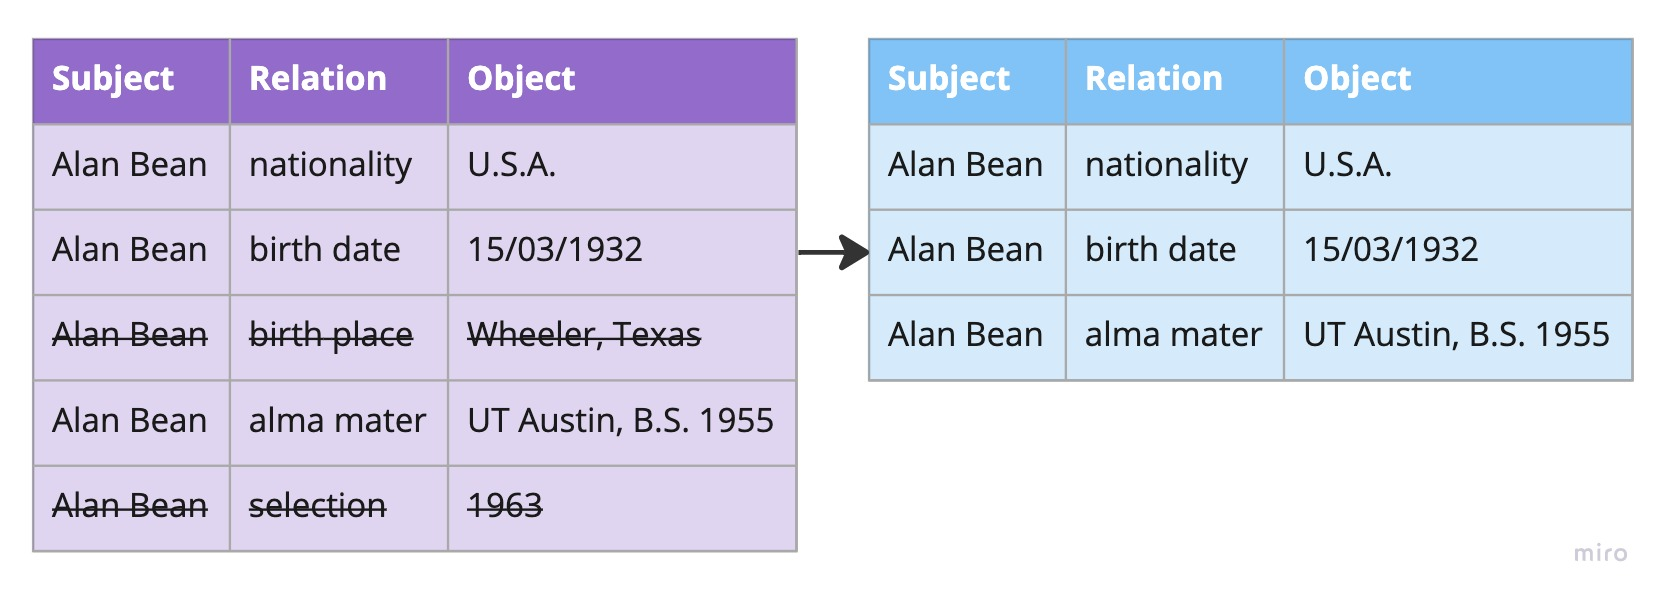
\includegraphics[scale=0.2]{figures/design/synthetic/hallu_graph.jpg}
    \caption{Phase (b). Synthetic hallucination graph generation, i.e. $\Tilde{G}$.}
    \label{fig:synthetic-hallu-graph}
\end{figure}

\begin{figure}
    \centering
    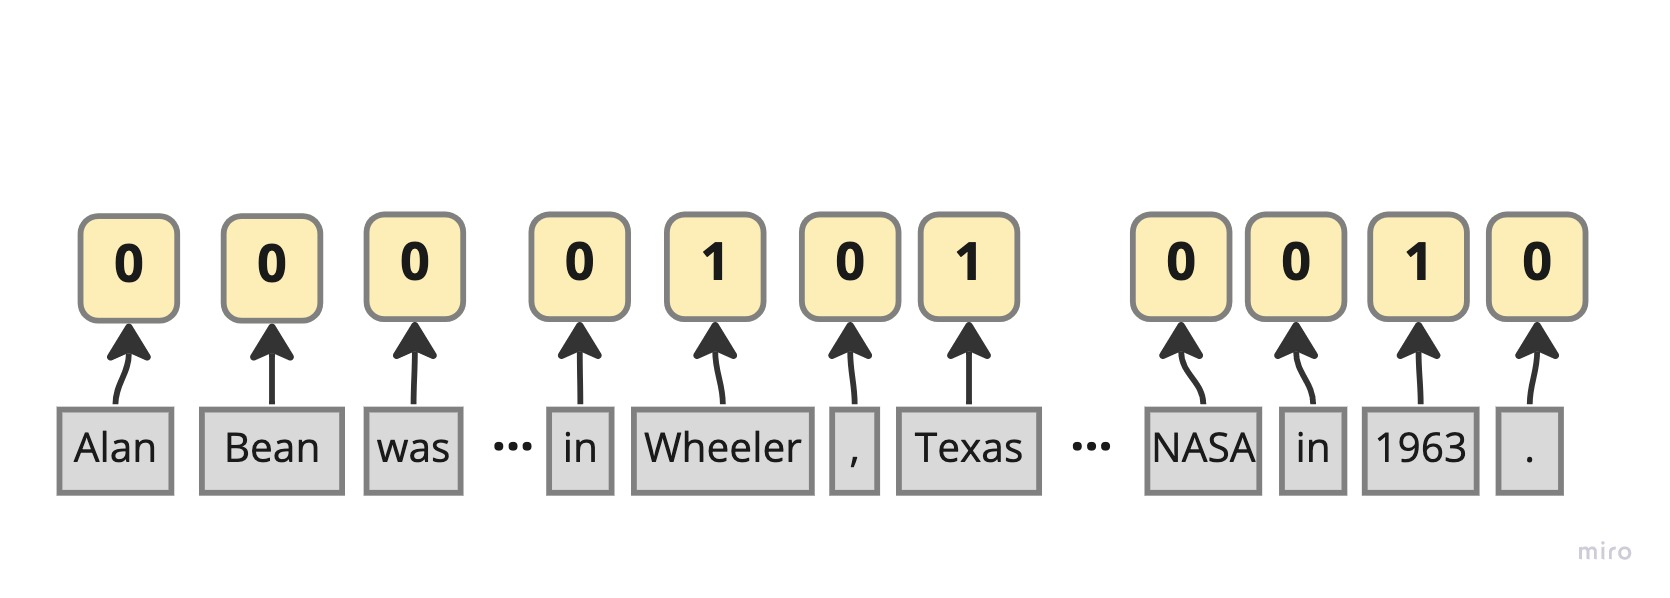
\includegraphics[scale=0.18]{figures/design/synthetic/hallu_labels.jpg}
    \caption{Phase (c). Synthetical hallucination labels generation, i.e. $\{a_j\}_j$.}
    \label{fig:synthetic-hallu-labels}
\end{figure}
\newpage
Based on $\Tilde{C}_G$, let $\Tilde{G} = \{e \in G \,:\, subject(e) \not\in \Tilde{C}_G \;\land\; object(e) \not\in \Tilde{C}_G\}$ be the graph containing only edges without hallucination. This constitutes the second step of the generation pipeline, and it can be visualised in figure \ref{fig:synthetic-hallu-graph}. Finally, the synthetic labels are defined as $a_{j} = I\{\exists_k \;:\; t_j \in c_k, \; c_k \in \Tilde{C_G}\}$ and are highlighted in figure \ref{fig:synthetic-hallu-labels}. This procedure can be generalised to all pairs $(G_i, T_i)$ so that $a_{i,j}$ corresponds to the hallucination label for the $j^{th}$ token of the $i^{th}$ text. It is also convenient to define the graph-to-text hallucination dataset $\Tilde{D} = \{(\Tilde{G_i}, T_i, a_{i, \cdot})\}_{i=1}^N$.

As a post-processing step, all hallucination labels $a_{i,j} = 1 $ corresponding to stop words are reset to non-hallucinations, i.e. $a_{i,j} = 0$. This ensures that hallucinations are only composed of pure expression of knowledge in the reference texts. For each $G_i$, $K$ is set so that roughly $1/3$ of the edges of the graph are dropped using this procedure.  

\subsection{Hallucination detection models} \label{design:hallucination-detection-models}
%Carefully chosen pieces of information are removed from the input graph to force models to generate hallucinations. 

The synthetic dataset described in section \ref{design:synthetic-hallucination-data} provides an extra set of labels for hallucination detection for graph-to-text. The latter can be used to analyse models trained to perform hallucination detection at token-level, i.e. for each token $t_j$ of each text $T_i$, a binary prediction $\hat a_{ij}$ has to be produced.

To this end, different hallucination detection approaches are compared. A detection baseline is constructed using the evaluation pipeline of Lee et al.\cite{factualityEnhancedLM} described in section \ref{related-work:factuality-enhanced-LM}. They use named-entity recognition to detect relevant factual information in the input graph and generated text. Furthermore, in a data-to-text use case, one can argue that the reference text should only contain factual information or expression of knowledge, e.g. no personal opinion or chitchat sentences. Hence, the check-worthy continuations identification step is less relevant here. In addition, the knowledge base can be restricted to the input data in graph-to-text applications. Particular emphasis is also placed on numeral hallucinations so that all text-like tokens (according to the spaCy library) in the prediction are considered valid expressions of knowledge and should therefore be checked for hallucination. Some efforts were made to reduce the number of false positives in their hallucination-checking phase by introducing a set of equivalents entities to be checked. For instance, shorter forms of country names and locations were not handled properly, e.g. USA, US, U.S.A., United States, similarly for quantities (e.g. 1 kg, 1000 g, 1.0 kg), dates (e.g. 17 June 2010, 17/06/2010, 17-06-2010), inhabitants and countries (e.g. Swiss, Switzerland), etc.   

The second hallucination detection model is directly based on the synthetic hallucination dataset. A logistic regression model is trained to detect hallucinations at token-level using entropy as the sole feature. The objective of this experiment is not to reach top-level performance but rather to quantify the predictive power of entropy for the hallucination detection task. Several variations of entropy as a feature are considered:
\begin{enumerate}
    \item Total entropy. It can be further decomposed into data and model uncertainty features to analyse which component has the strongest impact on hallucination occurrence. 
    \item Entropy of the $L$ previous tokens to introduce a dependence on past sequence elements. Since the hallucinations are synthesised at word-level and then expanded into tokens, one hallucination token is likely followed by a few additional ones. 
\end{enumerate}

For readability reasons, token-level predictions can also be aggregated at word-level using the following policy: a word is considered to be a hallucination if any of the tokens composing it is a hallucination. Given a predicted hallucination probability sequence $P = \{p_j\}_j$ corresponding to the tokens $T = \{t_j\}_j$, the word expansion of $P$, $\Tilde{P}$ is defined by 

$$
\Tilde{p_j} = \argmax_{t_l \in word(t_j)} p_l\;\;\; \forall\; j = 1, \ldots, L
$$
$$
words(t_j) = \{t_l \;:\; t_l \;\text{and}\; t_j \;\text{belong to the same word}\; \forall\;l=1,\ldots,L\}
$$

Since the hallucination labels $\hat a_{ij}$ are constructed at word-level, word expansion as a post-processing step for a token-level detection model is expected to increase its performance.